\documentclass[11pt,a4paper]{article}
\usepackage[margin=2.3cm]{geometry}
\usepackage{amsmath,amssymb,bm}
\usepackage{graphicx}
\usepackage{booktabs}
\usepackage[colorlinks=true,linkcolor=blue,citecolor=blue,urlcolor=blue]{hyperref}
\graphicspath{{../../results/}}
\setlength{\emergencystretch}{1.5em}

\newcommand{\Cg}{C_{\rm g}}
\newcommand{\Cl}{C_{\ell}}
\newcommand{\zr}{\zeta_r}
\newcommand{\zg}{\zeta_{\rm g}}
\newcommand{\dd}{\mathrm{d}}
\newcommand{\E}{\mathbb{E}}
\newcommand{\fnl}{f_{\rm NL}}
\newcommand{\fpbh}{f_{\rm PBH}}
\newcommand{\Mo}{M_\odot}
\newcommand{\Pz}{\mathcal{P}_\zeta}

\title{\textbf{Peaks or thresholds?}\\[6pt]
\Large Non-Gaussian primordial black hole abundances for broad spectra\\
and the pulsar-timing-array tension}
\author{Duong Ngoc Khoa\thanks{Phenikaa Institute for Advanced Study. ORCID 0009-0009-9409-3298.
Draft of 24 October 2026; the code \texttt{ngpbh} and every number below are in the accompanying
repository.}}
\date{}

\begin{document}
\maketitle

\begin{abstract}
The abundance of primordial black holes (PBHs) that accompanies an enhanced curvature spectrum
is computed either with threshold statistics or with peaks theory. With local
non-Gaussianity (NG), peaks theory had been applied only to monochromatic spectra or with the
peak condition imposed on a Gaussian field. We construct peaks theory on the compaction
function for broad spectra and local NG as the exact counterpart of threshold statistics, with
the same threshold, window, transfer function and cut-off. The maxima of the non-Gaussian linear
compaction $\Cl=F'(\zr)\Cg$ are the BBKS maxima of the Gaussian field $\Cg+\lambda\zr$ with
$\lambda=\Cl F''/F'^2$, times a rank-one Hessian factor that we compute exactly to first order.
An independent Monte Carlo and counts of maxima on $256^3$ Gaussian random fields confirm the
result; the Gaussian-peak approximation used so far miscounts peaks by up to 18\%. The required
amplitude ratio $R=A_*^{\rm peaks}/A_*^{\rm threshold}$ is 0.74--0.82 for $|\fnl|\le2$ and
lognormal widths $0.1\le\Delta\le2$. The NG dependence cancels almost completely in
$R/R_{\rm Gauss}$, to within $\pm4\%$ (16\% for a strong ultra-slow-roll tail). Propagated to
the NANOGrav 15-year data, peaks theory strengthens the exclusion of a scalar-induced
gravitational-wave explanation by 0.2--0.8$\sigma$ (0.4$\sigma$ in the BBKS normalisation), for
every NG template and spectral shape we consider. This is smaller than the effect of NG itself
for $|\fnl|\gtrsim1$. We also add the primordial-NG corrections to the induced GW spectrum. We
include all seven terms for local NG, validated against Adshead et al. They lower the significance
by up to $0.26\sigma$ for $|\fnl|\le2$ and leave the gap between the statistics unchanged. The
gap is comparable to three analysis choices that are rarely stated:
\begin{itemize}
\item the transfer function in the collapse threshold;
\item the normalisation of $\fpbh$ (the expression in common use overestimates $\fpbh$ by a
factor of 3--13);
\item the frequency range of the PTA fit.
\end{itemize}
We quantify all three.
\end{abstract}

\section{Introduction}

Pulsar timing arrays (PTAs) have found evidence for a nanohertz gravitational-wave background
\cite{NG15gwb}. One cosmological interpretation is the gravitational waves induced at second
order by a peak in the primordial curvature spectrum \cite{Ananda,Baumann,Kohri,Domenech,NG15np}.
A peak large enough to produce the signal also forms PBHs when the perturbations re-enter the
horizon. Requiring that PBHs are not overproduced disfavours the scenario at the 2--3$\sigma$
level \cite{FIVT23,NG15np,Iovino24}. How strongly depends on the NG of the curvature perturbation
and on how the PBH abundance is computed.

Two prescriptions are in use for the abundance:
\begin{itemize}
\item \textbf{Threshold statistics} counts the volume fraction in which the compaction function
exceeds a threshold. It includes the non-linear relation between curvature and density and any
local NG non-perturbatively \cite{Ferrante,Ianniccari}.
\item \textbf{Peaks theory} counts maxima \cite{BBKS}. It has been developed for Gaussian
curvature with finite width \cite{Pi25,Kushwaha,ColeFumagalli} and for local NG with
monochromatic spectra \cite{Young22,Kitajima,Inui}.
\end{itemize}
Several recent papers state that peaks theory with local NG for broad spectra is an open problem
\cite{Ianniccari,Iovino24,IPV25,Pi25,ColeFumagalli}. 2306.17149 \cite{FIVT23} add, in a
footnote, that peaks theory ``provides slightly smaller amplitudes'', so their threshold-statistics
bounds are conservative.

This note fills that gap and quantifies the footnote.
\begin{itemize}
\item \textbf{Construction} (Sec.~\ref{sec:stats}). We build peaks theory on the compaction
function for broad spectra with local NG (quadratic, logarithmic or ultra-slow-roll, and
curvaton templates). It is the exact counterpart of threshold statistics, so that the two differ
only by the peak condition.
\item \textbf{Main technical step.} We count maxima of the non-Gaussian compaction itself, a local
function of two correlated Gaussian fields, rather than of its Gaussian component. This differs
from the closest existing work \cite{Riccardi,Escriva26,Germani25}.
\item \textbf{The gap} (Sec.~\ref{sec:R}). We give the amplitude ratio $R(\Delta,{\rm NG})$ between
the statistics.
\item \textbf{PTA consequences} (Sec.~\ref{sec:pta}). We propagate the ratio to the significance
of the PBH-overproduction tension for NANOGrav 15, with every analysis choice stated and varied.
\item \textbf{NG in the induced GWs} (Sec.~\ref{sec:ngsigw}). We add the primordial-NG corrections to
the GW spectrum, which 2306.17149 neglect.
\item \textbf{Two pitfalls.} The second appears widely in the literature.
  \begin{itemize}
  \item 2306.17149 compute the collapse threshold without the radiation transfer function,
  although their formula includes it.
  \item The $\fpbh$ normalisation in common use is too large by a factor of 3--13.
  \end{itemize}
\end{itemize}

\section{Two statistics for the non-Gaussian compaction}\label{sec:stats}

\subsection{Local NG and the compaction function}

The curvature perturbation is $\zeta=F(\zg)$ with $\zg$ Gaussian and power spectrum $\Pz$. We use
three templates:
\begin{itemize}
\item quadratic, $F=\zg+\frac35\fnl\zg^2$;
\item ultra-slow-roll (USR), $F=-\mu_*\ln(1-\zg/\mu_*)$, which is $F=-\frac2\beta\ln(1-\frac\beta2\zg)$
of 2306.17149 with $\mu_*=2/\beta$ and has $\fnl=5/(6\mu_*)$ at second order;
\item the sudden-decay curvaton, $\zeta=\ln X(r_{\rm dec},\zg)$ \cite{Ferrante}.
\end{itemize}
At smoothing scale $r$ (the scale that re-enters the horizon at formation, $k=1/r$), define the
Gaussian fields
\begin{align}
\Cg(\bm x;r)&=\int\!\frac{\dd^3k}{(2\pi)^3}e^{i\bm k\cdot\bm x}\,\tfrac{2\Phi}{3}(kr)^2W(kr)T(kr)\,\zg(\bm k),\\
\zr(\bm x;r)&=\int\!\frac{\dd^3k}{(2\pi)^3}e^{i\bm k\cdot\bm x}\,W_s(kr)T(kr)\,\zg(\bm k),
\end{align}
with the top-hat $W(y)=3(\sin y-y\cos y)/y^3$, the shell $W_s(y)=\sin y/y$, the radiation transfer
function $T(y)=W(y/\sqrt3)$ and $\Phi=2/3$. All moments use a hard cut $kr<4.49$, which the
peak moments need for broad spectra; it changes threshold-statistics amplitudes by $\le2\%$. For
a spherical configuration $\Cg=-2\Phi r\zg'$, $\zr=\zg(r)$, and the linear and full compaction of
$\zeta=F(\zg)$ are \cite{Ferrante,Young22}
\begin{equation}
\Cl=F'(\zr)\,\Cg,\qquad C=\Cl-\frac{\Cl^2}{4\Phi}.
\label{eq:Cl}
\end{equation}
A PBH of mass $M=\mathcal K(C-C_{\rm th})^\gamma M_H$ forms where $C>C_{\rm th}$ and $\Cl<2\Phi$
(type I). We use $\mathcal K=3.3$ and $\gamma=0.36$. The threshold $C_{\rm th}=\delta_c(q)$ follows the
shape-dependent prescription of Musco et al. \cite{Musco21,EGS20}, with the transfer function
in the moments.

\subsection{Threshold statistics}
With $P_{\rm G}(c,z)$ the bivariate Gaussian of $(\Cg,\zr)$, the mass fraction at one scale is
\cite{Ferrante}
\begin{equation}
\beta_{\rm th}=\int\dd z\int_{C_{\ell,\rm th}}^{2\Phi}\dd\Cl\;\frac{P_{\rm G}(\Cl/F'(z),z)}{|F'(z)|}\;
\mathcal K(C-C_{\rm th})^\gamma ,
\label{eq:betath}
\end{equation}
where $C_{\ell,\rm th}=2\Phi[1-(1-C_{\rm th}/\Phi)^{1/2}]$. Equation~\eqref{eq:betath} includes the
non-linear $C(\Cl)$ and the full $F$.

\subsection{Peaks of the Gaussian component (Gaussian-peak approximation)}

The natural generalisation of earlier work is to count BBKS maxima of the Gaussian field $\Cg$,
with $\zr$ as a correlated scalar, and map them through $F'$. Where $F'<0$, maxima of $\Cl$ are
minima of $\Cg$. This replaces the volume weight in \eqref{eq:betath} by
\begin{equation}
w=\frac{V\,G(m,s)}{(2\pi)^{3/2}R_*^3},\qquad G(m,s)=\int_0^\infty\dd x\,f(x)\,\mathcal N(x;m,s^2),
\qquad V=\tfrac43\pi r^3,
\label{eq:3a}
\end{equation}
where:
\begin{itemize}
\item $f$ is the BBKS function \cite{BBKS};
\item $m$ and $s^2$ are the conditional mean and variance of $x=-\nabla^2\Cg/\sigma_{2}$ given
$(\Cg,\zr)$;
\item $R_*=\sqrt3\sigma_1/\sigma_2$.
\end{itemize}
This is exact for $F'=$ const, but not in general: $\nabla\Cl=F'\nabla\Cg+F''\Cg\nabla\zr$, so the
maxima of $\Cl$ are displaced from those of $\Cg$.

\subsection{Peaks of the non-Gaussian compaction}

The Kac--Rice density of maxima of $\Cl$ at $(\Cg,\zr)=(c,z)$ follows from three steps:
\begin{enumerate}
\item The gradient factorises:
\begin{equation}
\nabla\Cl=F'(z)\,\nabla Y_\lambda,\qquad Y_\lambda\equiv\Cg+\lambda\zr,\qquad \lambda=\frac{cF''(z)}{F'(z)},
\end{equation}
with $\lambda$ frozen at the point, so that $Y_\lambda$ is a Gaussian field.
\item At a stationary point, $\nabla\nabla\Cl=F'[\nabla\nabla Y_\lambda+\kappa\nabla\zr\nabla\zr^T]$,
with $\kappa=-cF'(1/F')''$. The rank-one term vanishes identically for the USR template, since
$1/F'$ is linear there.
\item Conditional on $\nabla Y_\lambda=0$, the gradient $\nabla\zr$ is Gaussian with variance
$v=(\sigma^2_{1,cc}\sigma^2_{1,rr}-\sigma^4_{1,cr})/(3\sigma^2_{1,\lambda})$. Here
$\sigma^2_{n,AB}=\int\dd\ln k\,k^{2n}K_AK_B\Pz$ and
$\sigma^2_{n,\lambda}=\sigma^2_{n,cc}+2\lambda\sigma^2_{n,cr}+\lambda^2\sigma^2_{n,rr}$.
\end{enumerate}
The determinant lemma then gives the peak density exactly to first order in $\tau=s\kappa
v/\sigma_{2,\lambda}$ (Appendix~\ref{app:3b}):
\begin{equation}
\boxed{\;n(c,z)=P_{\rm G}(c,z)\,\frac{G(s\,m_\lambda,s_\lambda)}{(2\pi)^{3/2}R_{*,\lambda}^3}\,
\big[1-\tau R_2(s\,m_\lambda,s_\lambda)\big],\qquad R_{*,\lambda}=\frac{\sqrt3\,\sigma_{1,\lambda}}{\sigma_{2,\lambda}},\;}
\label{eq:3b}
\end{equation}
with $s={\rm sign}\,F'$, $m_\lambda$ and $s_\lambda$ the conditional moments of
$-\nabla^2Y_\lambda/\sigma_{2,\lambda}$, and $R_2=27\int f_2\mathcal N/\int f\mathcal N\to9/m$. The peak
mass fraction is \eqref{eq:betath} with the integrand multiplied by $V n/P_{\rm G}$.
Equation~\eqref{eq:3b} has three limits:
\begin{itemize}
\item it reduces to \eqref{eq:3a} for $\lambda=0$ (Gaussian $\zeta$ or $F''=0$);
\item it reduces to \eqref{eq:3a} for a monochromatic spectrum, where $Y_\lambda\propto\zr$;
\item it is finite as $F'\to0$.
\end{itemize}
The rank-one factor is formally one power of the r.m.s.\ amplitude smaller, but
$\kappa=-2\lambda^2/c$ for the quadratic template. It changes the local density by up to 36\% at
nodes with $\fnl=-2$, $\Delta=1$.

\textbf{Checks.}
\begin{itemize}
\item An independent Monte Carlo of the 20 Gaussian variables with the exact Hessian reproduces
\eqref{eq:3b} to $3\times10^{-4}$ at 15 of 16 test nodes, and to 0.85\% at the most extreme one.
\item We counted local maxima of $\Cl$ on $256^3$ Gaussian random fields (lognormal $\Delta=1$,
24 realisations), with predictions from the lattices' own mode sums (Fig.~\ref{fig:lattice}).
Eq.~\eqref{eq:3b} follows the counts to about 1\% beyond the grid trend seen in the Gaussian
case. The Gaussian-peak approximation \eqref{eq:3a} is off by up to 18\% for $\fnl=-2$.
\end{itemize}

\begin{figure}[t]
\centering
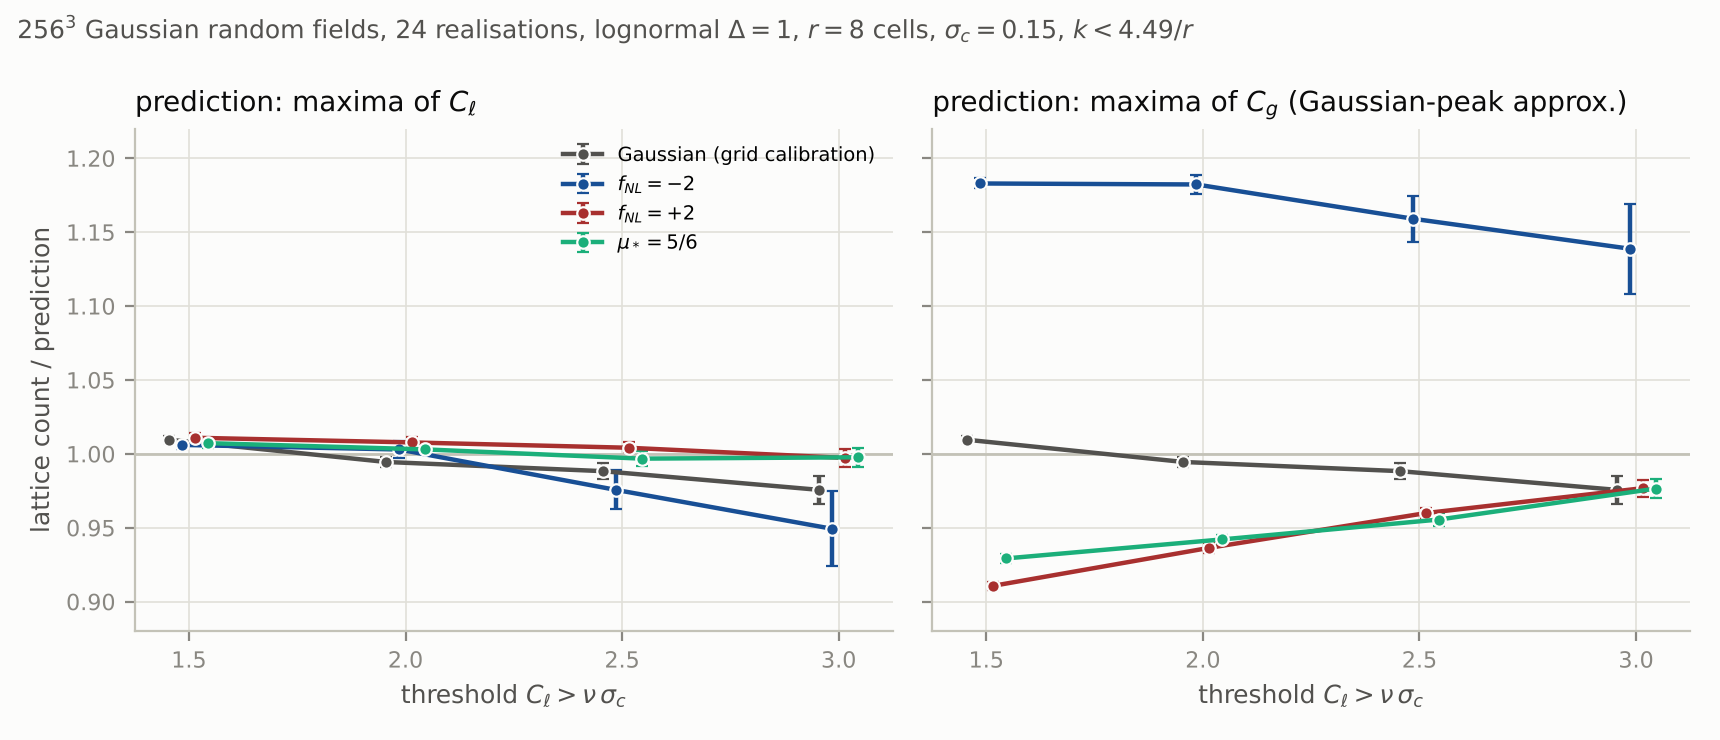
\includegraphics[width=0.86\textwidth]{fig_phase3b_lattice.png}
\caption{Maxima of $\Cl=F'(\zr)\Cg$ counted on $256^3$ Gaussian random fields, divided by the
prediction of eq.~\eqref{eq:3b} (left) and of the Gaussian-peak approximation \eqref{eq:3a}
(right), as a function of the threshold in units of $\sigma_c$. Gray: Gaussian $\zeta$, which
calibrates the grid.}
\label{fig:lattice}
\end{figure}

\section{Abundance and its conventions}\label{sec:abund}

The abundance integrates the mass fraction over the horizon mass $M_H$ at which $k=1/r$
re-enters:
\begin{equation}
\fpbh=\int\dd\ln M_H\;w(M_H)\,\beta(M_H).
\end{equation}
Three normalisations of $w$ are in use (Appendix~\ref{app:fpbh}):
\begin{itemize}
\item the $M_{\rm eq}$ form $w=(M_{\rm eq}/M_H)^{1/2}/\Omega_{\rm DM}$ \cite{Ferrante,ColeFumagalli};
\item eq.~(14) of 2306.17149, $w=(M_H/\Mo)^{-1/2}(g_*/106.75)^{3/4}(g_{*s}/106.75)^{-1}/(7.9\times10^{-10}\,\Omega_{\rm DM})$;
\item the first-principles result from entropy conservation, which is the same expression with
$1.0\times10^{-8}$ in place of $7.9\times10^{-10}$.
\end{itemize}
The first two overestimate $\fpbh$ by factors of 3--5 and 12.7 respectively. Since $\beta$
depends exponentially on $1/A$, this lowers the amplitude for $\fpbh=1$ by only
$\ln(\text{factor})/|\ln\beta|\simeq8\%$ and 12\%. These factors cancel in $R$ but not in the PTA
tension.

The threshold prescription is a second, larger choice. The Musco et al.\ shape parameter $q$
\cite{Musco21} depends on whether the transfer function enters its determination:
\begin{itemize}
\item for a lognormal of width $\Delta=1$, $\delta_c=0.537$ with it and $0.458$ without;
\item for the broken power law of 2306.17149 ($\alpha,\beta,\gamma=4,3,1$), $\delta_c=0.570$ and
$0.544$.
\end{itemize}
The thresholds in Fig.~S3 of 2306.17149 are the values without the transfer function. The
difference moves $A_*$ by 18\% (BPL) and 62\% (lognormal, $\Delta=1$), for every statistic,
because the linear threshold $C_{\ell,\rm th}$ grows faster than $C_{\rm th}$.

Our implementation \texttt{ngpbh} was validated as follows:
\begin{itemize}
\item it reproduces the public code \texttt{pbhstat} \cite{ColeFumagalli} in its conventions to
0.017\% in $A_*$ for $\Delta=0.1$--2, for both statistics;
\item it reproduces the broad-spectrum benchmark of Ferrante et al.\ (amplitude
$9.09\times10^{-3}$ vs $9.2\times10^{-3}$);
\item it reproduces their curvaton amplitudes to 1\% \cite{Ferrante}.
\end{itemize}
The integration uses Gauss--Legendre nodes in $\Cl$ that absorb the $(C-C_{\rm th})^\gamma$
cusp and an adaptive window in $\zr$, all in $\log\beta$. It is stable to $10^{-5}$ when every
grid is doubled.

\section{The gap between the statistics, with NG}\label{sec:R}

Table~\ref{tab:R} and Fig.~\ref{fig:R} give $R=A_*^{\rm peaks}/A_*^{\rm threshold}$ for
$\fpbh=1$, with the same threshold, window, transfer function, cut, $\mathcal K$ and $\gamma$ for
both statistics.
\begin{itemize}
\item \textbf{Gaussian $\zeta$:} $R=0.770$--$0.789$ in the BBKS normalisation with
$V=\frac43\pi r^3$.
\item \textbf{Conventions:} $R$ spans 0.75--0.89 across the normalisation conventions in use
(Press--Schechter factor, peak volume, Jacobian). It is about 0.6--0.67 with the high-peak
formula of Ref.~\cite{Iovino24} as used in Ref.~\cite{Blas26}. These conventions cancel to
better than 1\% in the double ratio $R/R_{\rm Gauss}$.
\item \textbf{The double ratio:} it stays within 0.958--1.036 for $|\fnl|\le2$. The strongly
non-perturbative USR tail $\mu_*=5/6$ reaches 1.05--1.16, the largest value at $\Delta=2$.
\item \textbf{True NG peaks vs the Gaussian-peak approximation:} the amplitudes differ by
$A^{\rm 3b}_*/A^{\rm 3a}_*=0.983$--1.000. The 18\% miscount of peaks moves $A_*$ by at most
1.7\%, because $\delta\ln A_*\simeq\delta\ln n/|\ln\beta|$.
\end{itemize}
For comparison, NG moves the threshold-statistics amplitude itself by factors of 0.2--2 over the
same grid.

\begin{table}[t]
\centering\small
\begin{tabular}{lccccc}
\toprule
template & $\Delta=0.1$ & $0.3$ & $0.5$ & $1$ & $2$\\
\midrule
Gaussian & 0.770 & 0.775 & 0.778 & 0.783 & 0.789\\
$\fnl=-2$ & 0.738 & 0.744 & 0.769 & 0.794 & 0.810\\
$\fnl=-1$ & 0.748 & 0.751 & 0.760 & 0.784 & 0.803\\
$\fnl=+1$ & 0.788 & 0.792 & 0.796 & 0.803 & 0.811\\
$\fnl=+2$ & 0.796 & 0.800 & 0.803 & 0.809 & 0.817\\
USR $\mu_*=5/6$ & 0.808 & 0.816 & 0.825 & 0.851 & 0.914\\
USR $\mu_*=5/2$ & 0.779 & 0.785 & 0.789 & 0.797 & 0.809\\
\bottomrule
\end{tabular}
\caption{$R=A_*^{\rm peaks}/A_*^{\rm threshold}$ with peaks of the non-Gaussian compaction
\eqref{eq:3b}, lognormal spectra of width $\Delta$, $\fpbh=1$, $k_*=10^7\,{\rm Mpc}^{-1}$.}
\label{tab:R}
\end{table}

\begin{figure}[t]
\centering
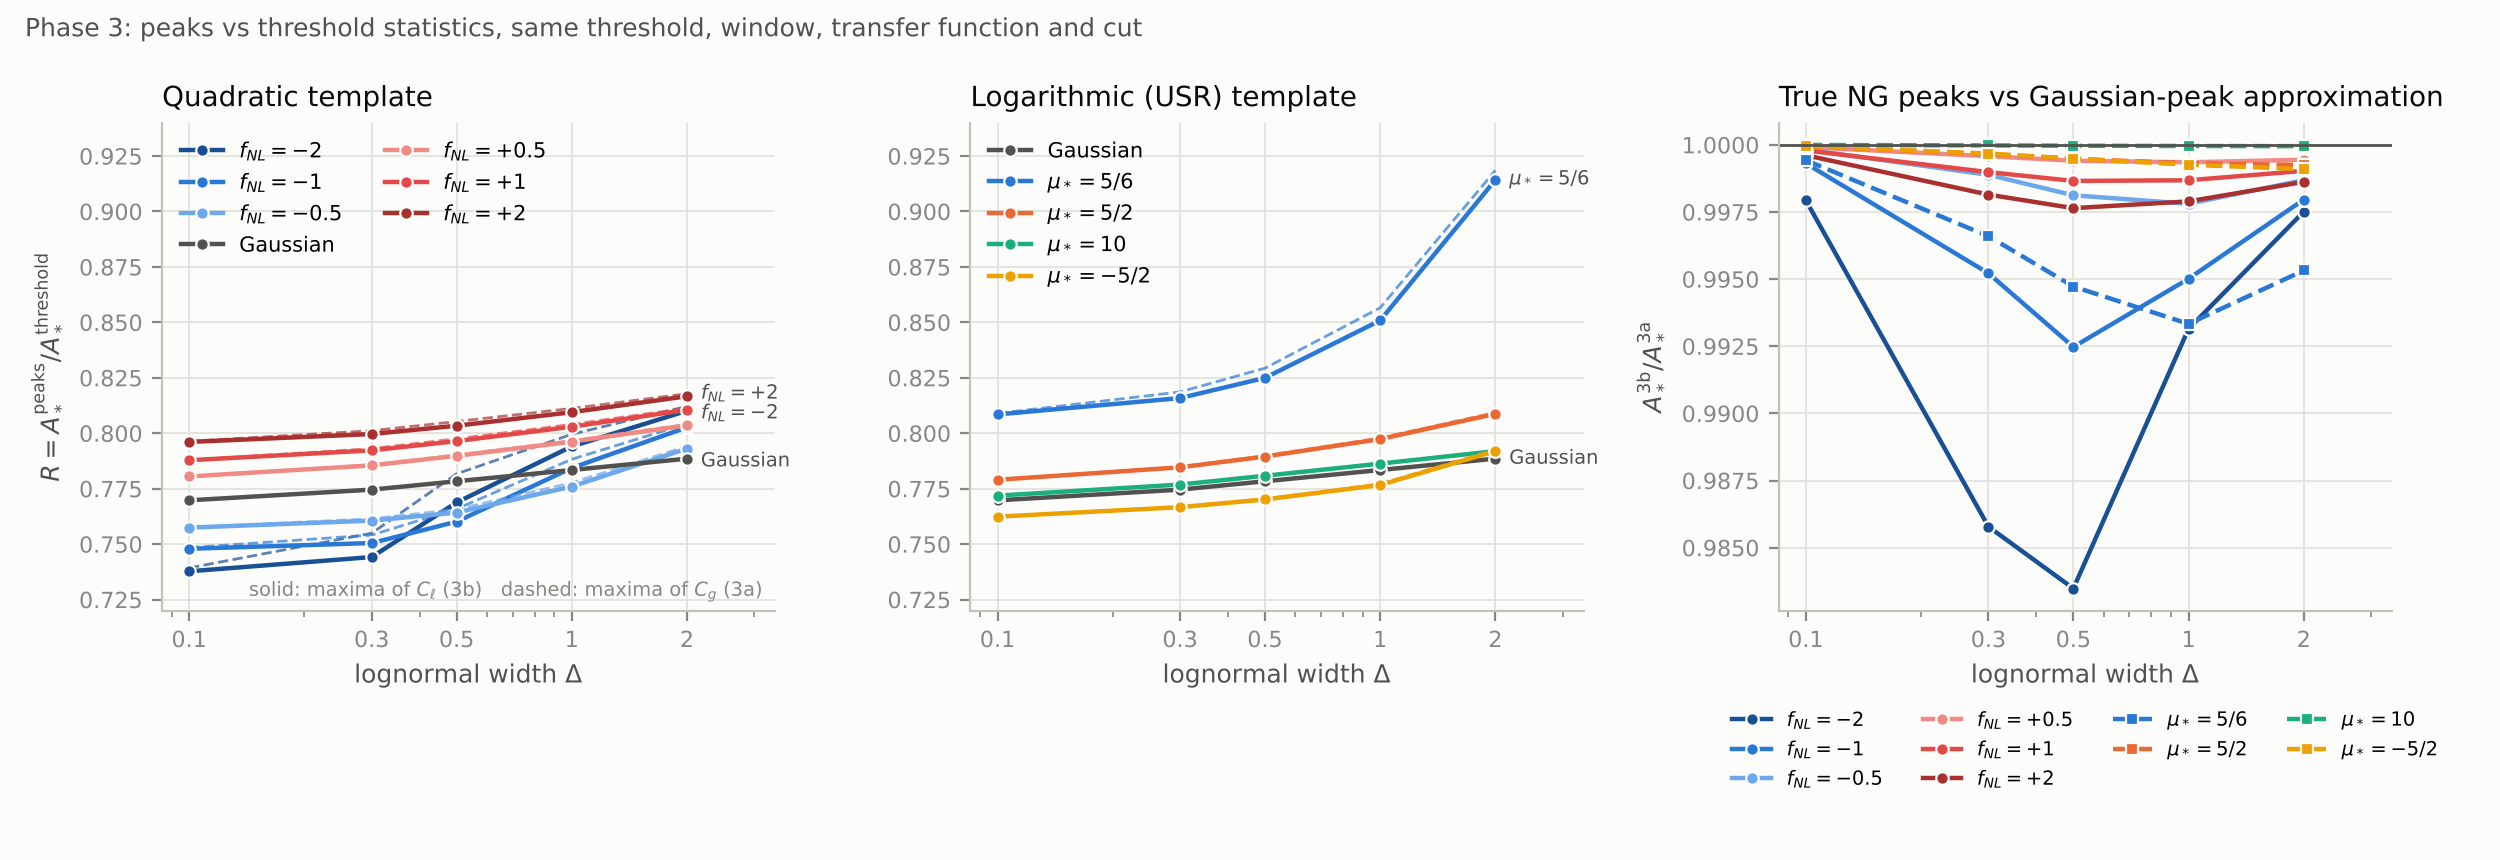
\includegraphics[width=\textwidth]{fig_phase3_ratio.png}
\caption{Left and middle: $R$ for the quadratic and logarithmic templates; solid lines are peaks
of $\Cl$ \eqref{eq:3b}, dashed lines are the Gaussian-peak approximation \eqref{eq:3a}. Right:
$A_*^{\rm 3b}/A_*^{\rm 3a}$.}
\label{fig:R}
\end{figure}

\section{Consequences for the PTA tension}\label{sec:pta}

\subsection{Gravitational waves and the NANOGrav 15 likelihood}

\textbf{Induced GWs.} For Gaussian $\zeta$ in radiation domination
\cite{Kohri,Espinosa,FIVT23},
\begin{equation}
\Omega_{\rm GW,RD}(k)=\frac16\int_1^\infty\!\dd t\int_0^1\!\dd s\left[\frac{(t^2-1)(1-s^2)}{t^2-s^2}\right]^2
I^2_{t,s}\;\Pz\!\Big(k\frac{t+s}{2}\Big)\Pz\!\Big(k\frac{t-s}{2}\Big),
\end{equation}
\begin{equation}
h^2\Omega_{\rm GW}(f)=h^2\Omega_r\,\frac{g_*}{g_*^0}\Big(\frac{g_{*s}}{g_{*s}^0}\Big)^{-4/3}\Omega_{\rm GW,RD}(k),
\end{equation}
with $f=k/2\pi$, $h^2\Omega_r=4.2\times10^{-5}$ and the Standard-Model $g_*(T)$ of \cite{Saikawa}.
The kernel is \cite{Kohri,FIVT23}
\begin{equation}
I^2_{t,s}=\frac{288(s^2+t^2-6)^2}{(t^2-s^2)^6}\left[\frac{\pi^2}{4}(s^2+t^2-6)^2\Theta(t-\sqrt3)
+\Big(t^2-s^2-\tfrac12(s^2+t^2-6)\ln\Big|\frac{t^2-3}{3-s^2}\Big|\Big)^2\right].
\end{equation}
We rewrite the logarithmic bracket as $(3-s^2)\,g(e)$ with $e=(t^2-s^2)/(3-s^2)$ and
$g=-e^3/12-e^4/12-\dots$, so that the cancellation at $t,s\to1$ is done analytically. We also
split $t$ at the resonance $t=\sqrt3$.
Checks:
\begin{itemize}
\item a flat spectrum gives $0.8222436\,A^2$ \cite{Kohri};
\item the Dirac closed form is recovered;
\item direct two-dimensional integration agrees to $10^{-8}$--$10^{-12}$;
\item the infrared $k^3$ tail matches its asymptotic form.
\end{itemize}
This is the spectrum for Gaussian $\zeta$, as in \cite{FIVT23}; Sec.~\ref{sec:ngsigw} adds the
primordial-NG corrections.

\textbf{Likelihood.} We use the NANOGrav 15-year free spectrum with Hellings--Downs correlations
(the lowest 14 bins), represented by kernel density estimates of the per-bin posteriors in
$\log_{10}\rho$ \cite{Lamb,PTArcade}:
\begin{equation}
\ln L=\sum_j\ln p_j(\log_{10}\rho_j),\qquad
\rho_j^2=\frac{H_{100}^2\,h^2\Omega_{\rm GW}(f_j)}{8\pi^4f_j^5T},\qquad T=16.03\,{\rm yr}.
\end{equation}
The KDEs use a compact kernel with bandwidths down to 0.004 dex. Outside the sampled range their
density is floored, and their sparse tails are combs of single-sample spikes. We therefore
regularise them by taking the maximum of each density and its 0.05-dex Gaussian blur
(Appendix~\ref{app:kde}). This leaves the bulk unchanged and moves every significance below by
$\le0.14\sigma$.

\textbf{Validation of the likelihood:}
\begin{itemize}
\item for $h_c\propto f^{-2/3}$ it gives $A=2.52^{+0.59}_{-0.61}\times10^{-15}$ (90\%), against
$2.4^{+0.7}_{-0.6}\times10^{-15}$ from NANOGrav \cite{NG15gwb};
\item with a free slope it gives $\gamma=3.07^{+0.63}_{-0.56}$, against $3.2\pm0.6$;
\item for the lognormal SIGW fit with $\Delta$ marginalised it gives
$\log_{10}A=-0.57^{+0.54}_{-0.84}$, against $-0.56^{+0.53}_{-0.74}$ in 2306.17149;
\item for the broken power law with the shape marginalised it gives
$\log_{10}A=-0.84^{+0.79}_{-0.74}$, against $-0.86^{+0.79}_{-0.65}$, and $\log_{10}k_*=7.95$ against 7.92.
\end{itemize}

\textbf{Significance.} The posterior is taken in $(\log_{10}k_*,\log_{10}A)$, uniform on
$[5,10]\times[-3,0]$, for the same spectral shape as the PBH line. The ``allowed region'' is
$A<A_*(k_*)$, where $\fpbh(A_*)=1$. We quote two measures:
\begin{itemize}
\item $\sigma_P$, the one-sided Gaussian equivalent of the posterior mass in the allowed region;
\item $\sigma_{\rm HPD}$, the two-sided equivalent of the highest-posterior-density level at
which the region is first reached. This is the definition of 2306.17149: their
$1\sigma/2\sigma/3\sigma$ contours lie at our 69/94/99\% levels.
\end{itemize}
$\sigma_{\rm HPD}$ saturates on local features of a lumpy posterior ridge, so we lead with
$\sigma_P$. Values above $4\sigma$ lie where the KDEs carry no information and are quoted only
as ``$>4$''. The lines $A_*(k_*)$ for all $k_*$ come from one set of $\beta$ grids, because the
moments depend on $kr$ only.

\subsection{Reproducing 2306.17149}

Figure~\ref{fig:valid} compares our threshold-statistics bands with Fig.~3 of 2306.17149, read
exactly from the vector paths of the arXiv source. Their setup reproduces their bands only with
two of their unstated conventions: the threshold without the transfer function and their $\fpbh$
normalisation. With both, the agreement for $k_*\ge10^{7.5}\,{\rm Mpc}^{-1}$ is:
\begin{itemize}
\item Gaussian (non-linearities only): 1--6\% in $A$;
\item $\fnl=-2$: within 6\%;
\item USR with $\beta=3$: within 2.3\%;
\item curvaton $r_{\rm dec}=0.9$: 8--11\%.
\end{itemize}
Their bands dip by up to 0.05 dex near $k_*\simeq10^{6.5}$, where they include the QCD softening
of the formation parameters and we do not. Putting their own lines on our posterior changes the
significance by $\le0.07\sigma$, so the QCD omission does not matter, as they state.

\begin{figure}[t]
\centering
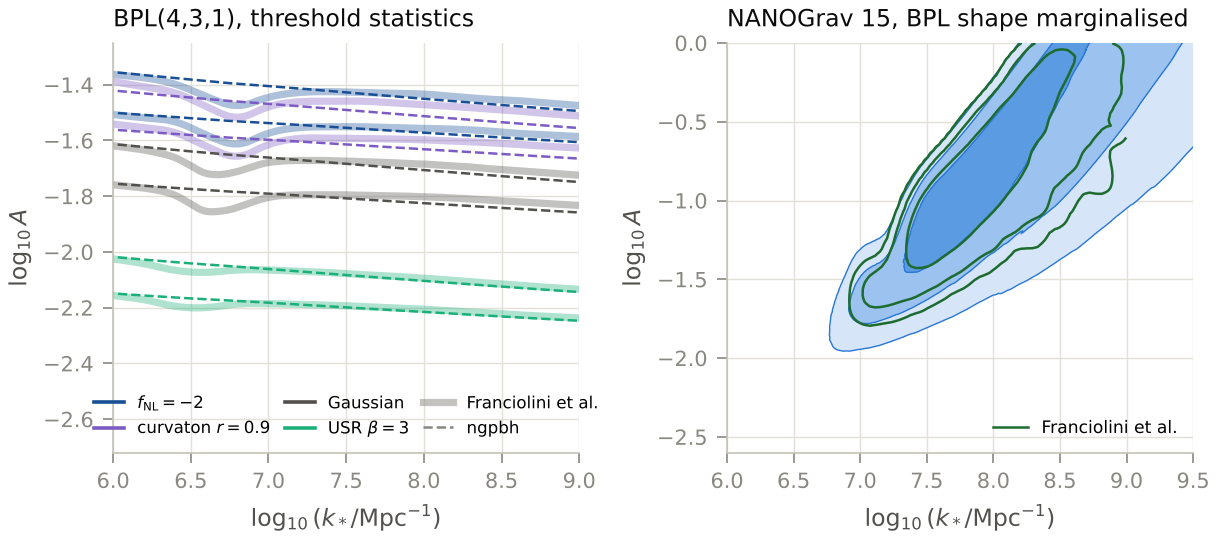
\includegraphics[width=\textwidth]{fig_phase5_validation.png}
\caption{Left: threshold-statistics bands $\fpbh=1$ (upper) and $10^{-3}$ (lower) for BPL(4,3,1);
wide lines are 2306.17149 Fig.~3 (with QCD), dashed lines are \texttt{ngpbh} (no QCD). Right: the
NANOGrav 15 posterior with the BPL shape marginalised (fill: 68.3/95.4/99.7\% HPD) and the
contours of 2306.17149.}
\label{fig:valid}
\end{figure}

\subsection{Exclusion per statistic and NG template}

Table~\ref{tab:pta} gives $\sigma_P$ for threshold statistics and for peaks of the non-Gaussian
compaction, in the conventions of 2306.17149. Figure~\ref{fig:sigma} shows all templates.
\begin{itemize}
\item \textbf{The statistics shift.} Over the 81 cases with $\sigma_P\le4$, peaks theory adds
$\Delta\sigma_P=+0.24$ to $+0.78$ (median $+0.42$). The amplitude shift itself is nearly uniform:
$-0.07$ to $-0.11$ dex, and $-0.05$ for the strongest USR tail at $\Delta=2$. It translates into
different $\Delta\sigma$ depending on where the line meets the posterior.
\item \textbf{Their setup.} With the shape-marginalised posterior and the BPL(4,3,1) lines, the
Gaussian case goes from $2.3$ to $2.8\sigma_P$ ($1.4$ to $1.9\sigma_{\rm HPD}$). $\fnl=-2$ goes from
$1.6$ to $1.9\sigma_P$, and the curvaton from $1.7$ to $2.0\sigma_P$. The USR $\beta=3$ case,
which they place beyond $3\sigma$, gives $3.9\sigma_P$ with threshold statistics and $>4$ with
peaks.
\item \textbf{True NG peaks vs the Gaussian-peak approximation.} They agree to $|\Delta\sigma_P|\le0.04$.
\item \textbf{The NG shift.} Relative to the Gaussian case it runs from $-1.2\sigma$ (negative
$\fnl$ and the curvaton, for narrow spectra) to well beyond $+2\sigma$ (positive $\fnl$ and USR
tails). For $\Delta=2$ the sign of the $\fnl<0$ shift flips, because large negative $\zg$ also
produce large compaction.
\end{itemize}

\begin{table}[t]
\centering\small
\begin{tabular}{lcccc}
\toprule
template & BPL(4,3,1) & LN $\Delta=0.5$ & LN $\Delta=1$ & LN $\Delta=2$\\
\midrule
Gaussian & 2.98\,$\to$\,3.62 & 3.02\,$\to$\,3.52 & 3.54\,$\to$\,$>4$ & 3.84\,$\to$\,$>4$\\
$\fnl=-2$ & 1.87\,$\to$\,2.18 & 1.88\,$\to$\,2.31 & 3.43\,$\to$\,3.84 & $>4$\\
$\fnl=-1$ & 1.98\,$\to$\,2.40 & 1.90\,$\to$\,2.36 & 3.05\,$\to$\,3.46 & 3.89\,$\to$\,$>4$\\
$\fnl=-0.5$ & 2.25\,$\to$\,2.93 & 2.22\,$\to$\,2.89 & 3.09\,$\to$\,3.51 & 3.60\,$\to$\,$>4$\\
$\fnl=+0.5$ & 3.67\,$\to$\,$>4$ & 3.60\,$\to$\,$>4$ & $>4$ & $>4$\\
curvaton $r_{\rm dec}=0.9$ & 2.01\,$\to$\,2.44 & 2.00\,$\to$\,2.43 & 3.09\,$\to$\,3.49 & 3.91\,$\to$\,$>4$\\
USR $\mu_*=5/2$ & 3.53\,$\to$\,$>4$ & 3.49\,$\to$\,3.91 & $>4$ & $>4$\\
$\fnl\ge+1$, USR $\mu_*\le5/6$ & $>4$ & $>4$ & $>4$ & $>4$\\
\bottomrule
\end{tabular}
\caption{Exclusion of the PBH-allowed region by NANOGrav 15, $\sigma_P$, threshold statistics
$\to$ peaks of $\Cl$ \eqref{eq:3b}, $\fpbh=1$. Conventions of 2306.17149 (threshold without the
transfer function, their $\fpbh$ normalisation); fixed spectral shape in both the line and the
posterior.}
\label{tab:pta}
\end{table}

\begin{figure}[t]
\centering
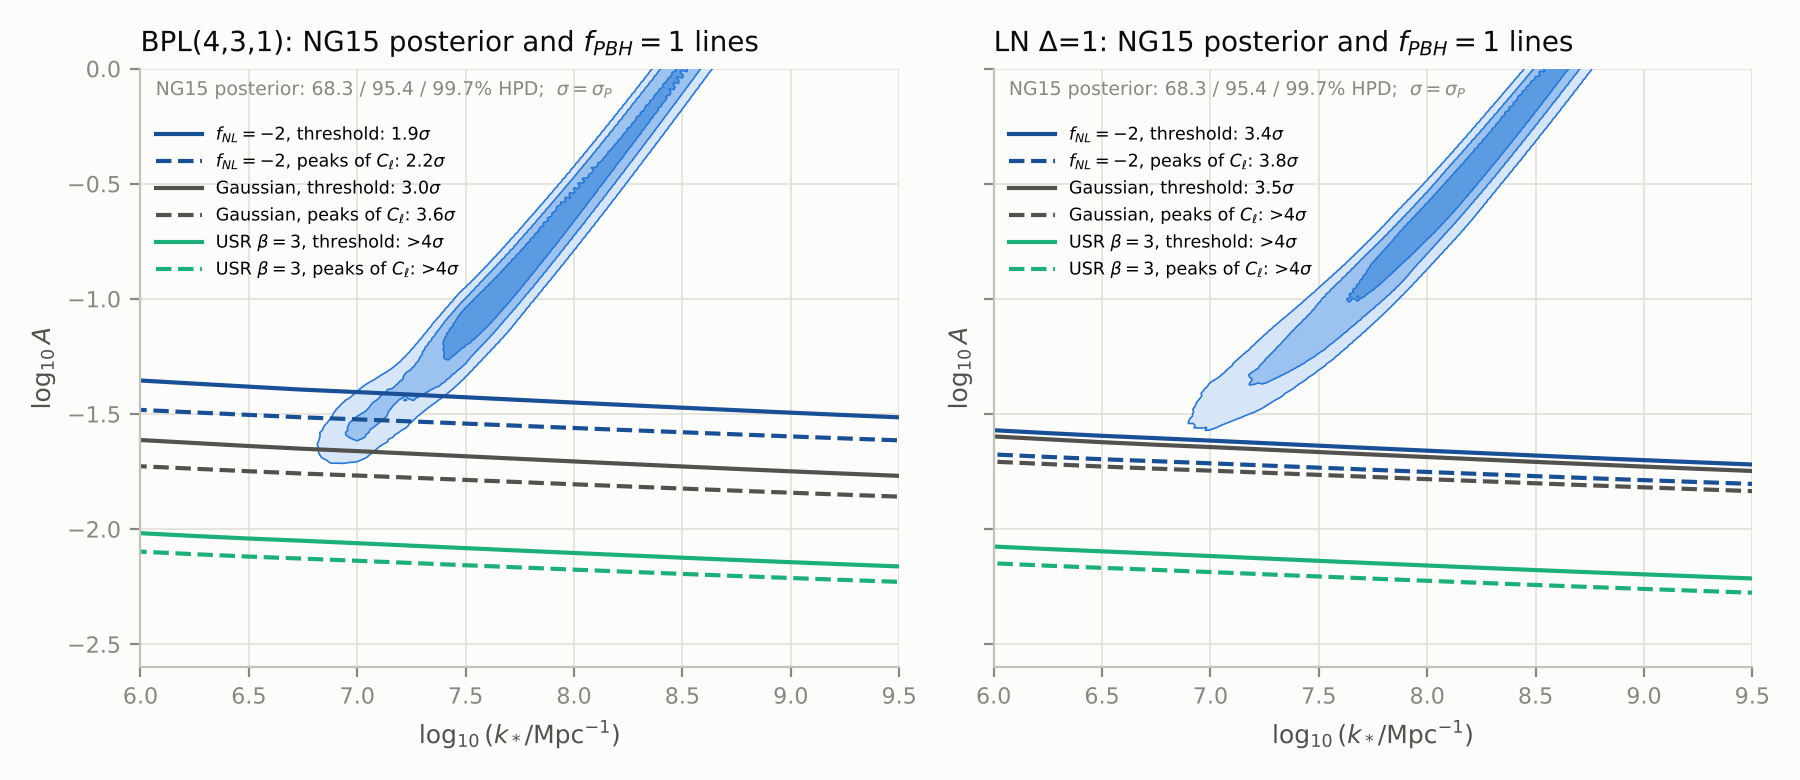
\includegraphics[width=\textwidth]{fig_phase5_tension.png}
\caption{NANOGrav 15 posteriors (68.3/95.4/99.7\% HPD) for BPL(4,3,1) and a lognormal of width 1,
with the $\fpbh=1$ lines from threshold statistics (solid) and peaks of $\Cl$ (dashed) for three
NG templates. The legend gives $\sigma_P$.}
\label{fig:tension}
\end{figure}

\begin{figure}[t]
\centering
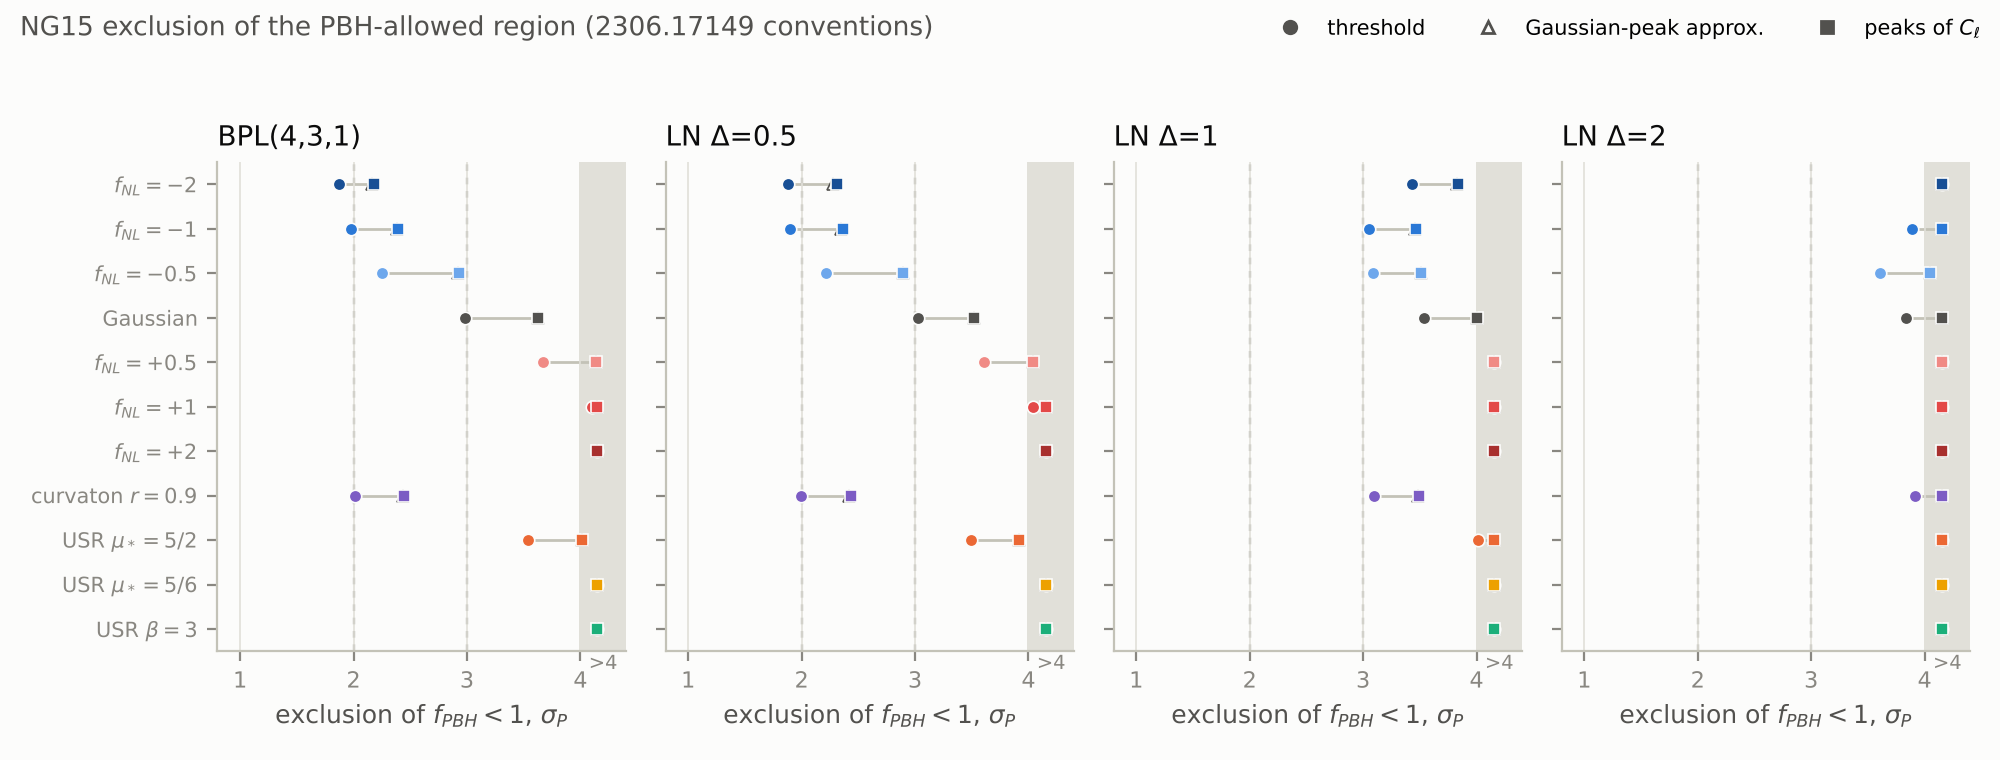
\includegraphics[width=\textwidth]{fig_phase5_sigma.png}
\caption{$\sigma_P$ per NG template for threshold statistics (circles), the Gaussian-peak
approximation (open triangles, hidden behind the squares) and peaks of $\Cl$ (squares).
Shaded: beyond $4\sigma$.}
\label{fig:sigma}
\end{figure}

\subsection{Primordial NG in the induced GWs}\label{sec:ngsigw}

So far the GW spectrum is that of Gaussian $\zeta$, as in 2306.17149. For the quadratic template
$\zeta=\zg+F(\zg^2-\langle\zg^2\rangle)$ with $F=3\fnl/5$, the four-point function of $\zeta$ ends at
$F^4$. The spectrum then has seven terms \cite{ALW21}:
\begin{equation}
\Omega_{\rm GW,RD}=A^2T_2+F^2A^3\,(T_{\rm hyb}+T_C+T_Z)+F^4A^4\,(T_{\rm red}+T_{\rm pl}+T_{\rm np}).
\end{equation}
For $\Pz^{\rm g}=A\,s(k/k_*)$ each term depends on $k/k_*$ only, and $A$ is the amplitude of the
Gaussian component, as in the PBH lines. All seven follow from
\begin{equation}
\Omega_X=\frac{k^3c_X}{12\pi^2}\int\prod_{\rm loops}\frac{\dd^3q}{(2\pi)^3}\,
{\rm Re}\big[z_1^2\bar z_2^2\big]\,J_{12}\prod_iP(|\bm m_i|),\qquad
J_{12}=\tfrac12\big(I_{A1}I_{A2}+I_{B1}I_{B2}\big).
\end{equation}
Here $z=(q_x+iq_y)/k$ is the transverse momentum of a GW vertex ($\bm k=k\hat z$). $J_{12}$ is the
oscillation average of the product of the late-time transfer functions
$I=(I_A\sin x+I_B\cos x)/x$ of the two vertices \cite{Kohri}; $J_{11}$ is the kernel above. The
$\bm m_i$ are the momenta that carry a power spectrum, $P(m)=2\pi^2\Pz^{\rm g}(m)/m^3$, and $c_X=2$,
8, 16, 16, 8, 32, 16 for the Gaussian, hybrid, C, Z, reducible, planar and nonplanar terms. These
reproduce the prefactors $2^5$, $2^7F^2$, $2^8F^2$, $2^8F^2$, $2^7F^4$, $2^9F^4$, $2^8F^4$ of
Ref.~\cite{ALW21}.

\textbf{Numerics.}
\begin{itemize}
\item \textbf{Disconnected terms.} They are the Gaussian functional of $P_{\rm g}+P_2$, with the
one-loop spectrum $\Pz^{(2)}=F^2A^2s_2$. We compute $T_{\rm hyb}=2\,\Omega_{\rm bil}[s,s_2]$ and
$T_{\rm red}=\Omega_{\rm G}[s_2]$ with the quadrature above.
\item \textbf{Connected terms.} These are five- and eight-dimensional; we use randomised
quasi-Monte Carlo over the spectral momenta. $L$ of the $L+1$ momenta $\bm m_i$ are drawn from
the spectrum, and the last follows from momentum conservation. The choices of which momentum is
fixed are combined with the balance heuristic, so the weights stay bounded when a momentum
becomes soft.
\item \textbf{Variance for broad spectra.} Here pairs of nearly independent vertices dominate the
variance: ${\rm Re}[z_1^2\bar z_2^2]\propto\cos2\phi$ averages to zero but scatters. We average
each sample over rotations about $\bm k$ of one spectral momentum (for the planar term, of two,
independently). The rotations preserve the measure and every weight, so the estimate stays
unbiased; the oscillation cancels.
\end{itemize}

\textbf{Checks.}
\begin{itemize}
\item The Monte Carlo reproduces the quadrature of the Gaussian, hybrid and reducible terms: 72
comparisons, rms pull 0.97.
\item All six NG terms agree with Fig.~4 of Ref.~\cite{ALW21}, read from the vector paths of the
arXiv source (Fig.~\ref{fig:ngvalid}). For lognormal widths 1/5 and 1/10 the agreement is within
3\% of each curve's maximum, including the sign changes of $T_Z$ and the negative $T_{\rm np}$.
\end{itemize}

\textbf{Other templates.} For $\zeta=\zg+F\zg^2+G\zg^3+\dots$, only $F$ and $G$ enter at
$O(A^3)$. $G$ enters through the power renormalisation $P\to(1+6G\sigma^2)P$, i.e.\
$+12G\sigma^2A^2T_2$; the $g_{\rm NL}$-type trispectrum vanishes under the azimuthal integral
\cite{Perna24}. $O(A^4)$ would need $G^2$, $F^2G$ and $FH$ terms, so we truncate the curvaton
($F=-0.62$, $G=0.32$ \cite{SVW06}) and the USR maps ($F=1/2\mu_*$, $G=1/3\mu_*^2$) at $A^3$. The
quadratic template is exact at $A^4$.

\begin{figure}[t]
\centering
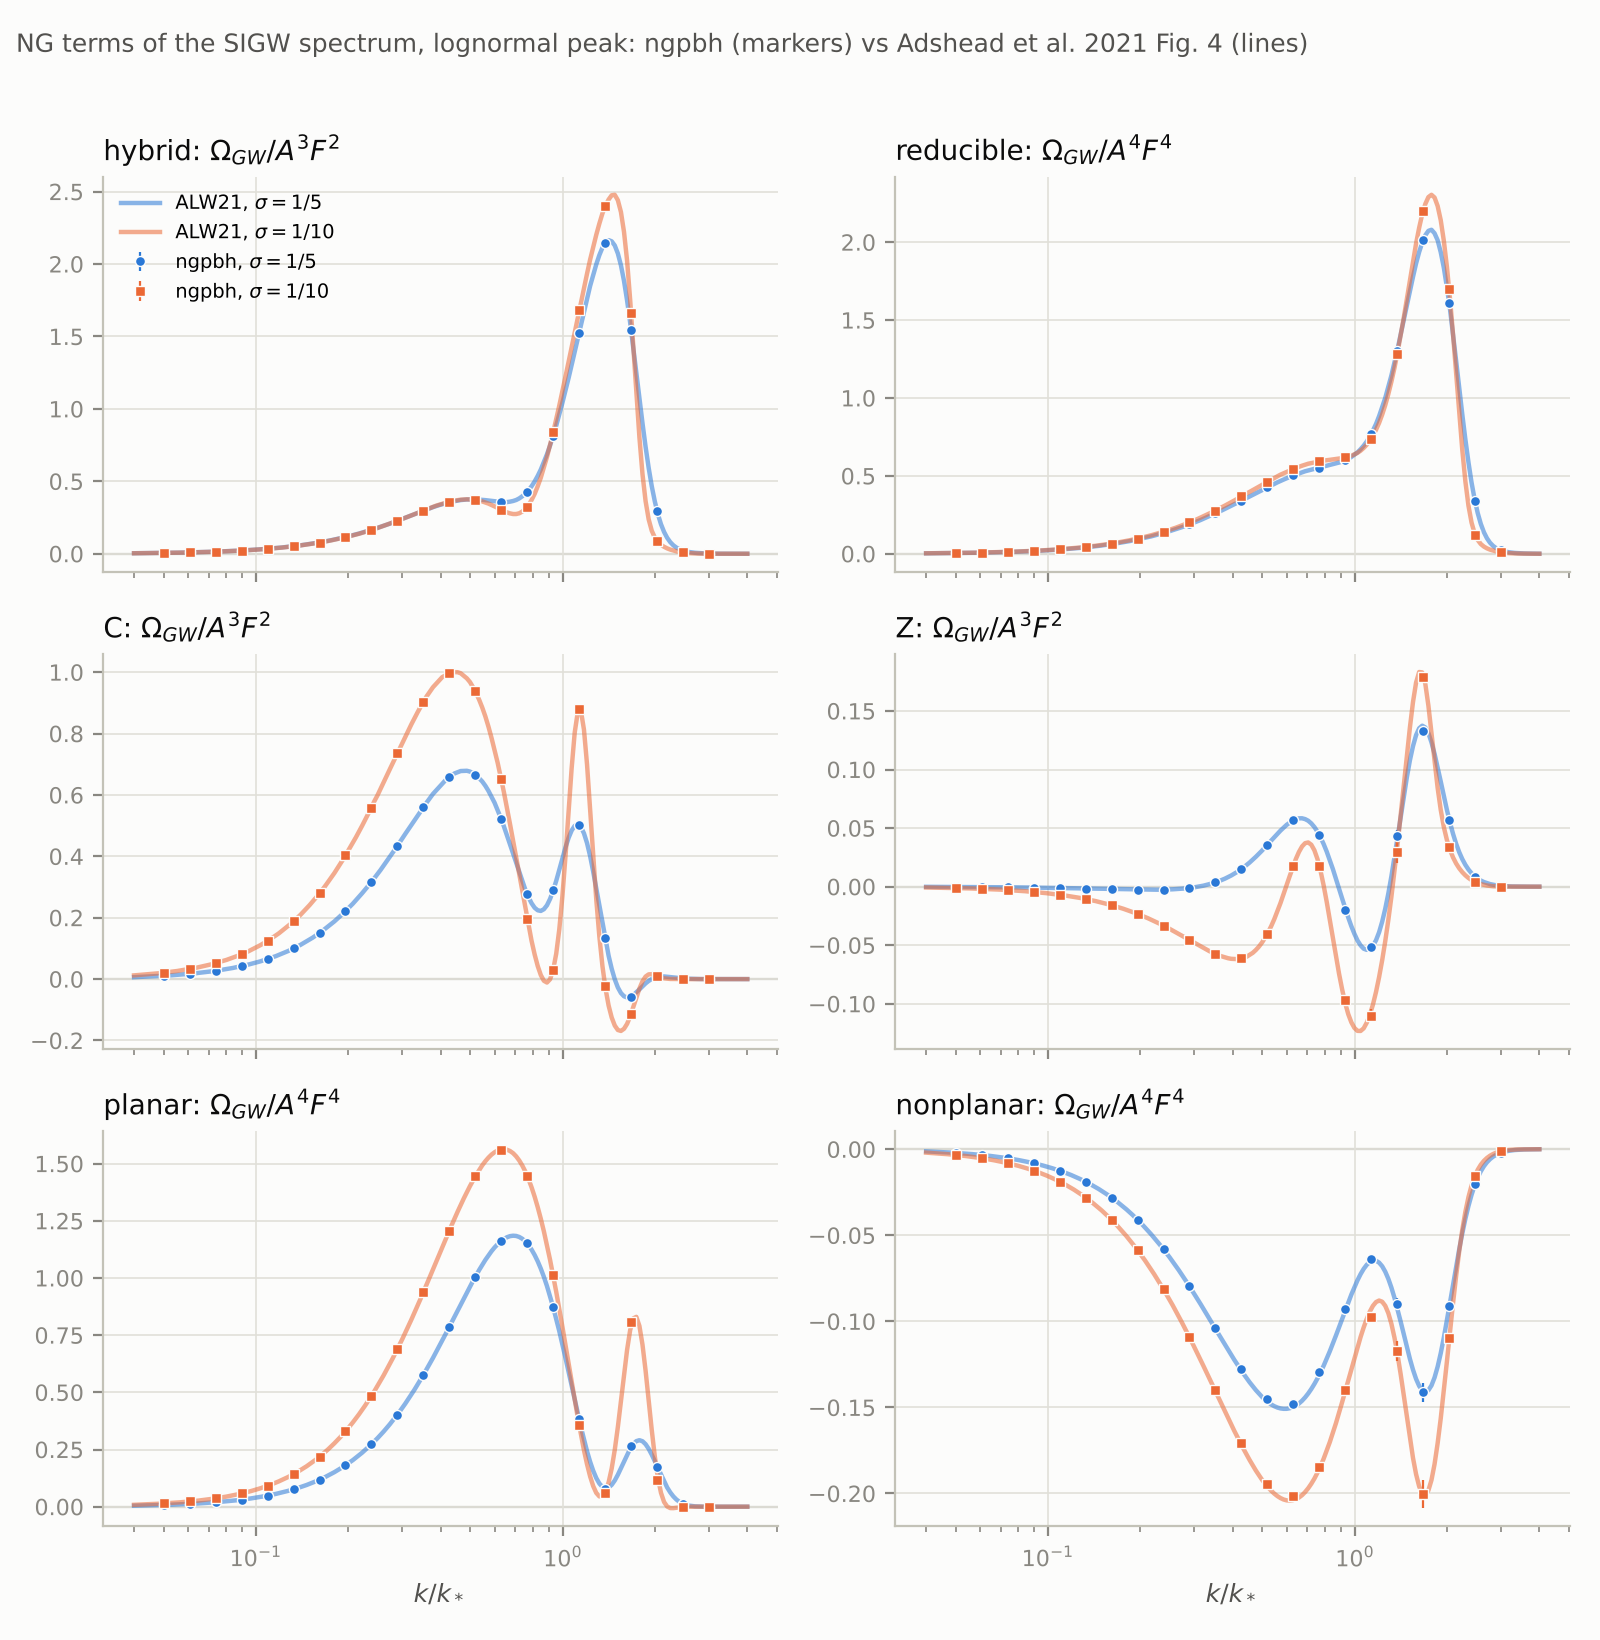
\includegraphics[width=0.84\textwidth]{fig_sigw_ng_validation.png}
\caption{The six NG terms of the induced GW spectrum for lognormal peaks ($A=F=1$):
\texttt{ngpbh} (markers, Monte Carlo errors smaller than the markers) against Fig.~4 of
Adshead, Lozanov \& Weiner \cite{ALW21} (lines, read from the vector paths of the arXiv
source).}
\label{fig:ngvalid}
\end{figure}

\textbf{Size.} Relative to $T_2$ the corrections are large (Fig.~\ref{fig:ngterms}). In the
NANOGrav band of the posterior bulk, $k/k_*\simeq0.02$--0.3, the ratio $T_3/T_2$ is 2--6. It grows
with the width of the peak, because the one-loop spectrum collects the whole variance
$\sigma^2=A$ while the peak value of a broad lognormal is low. For $|\fnl|=2$, $\Omega_{\rm GW}$ at
fixed $A$ is therefore 10--40\% larger near the PBH lines ($A\simeq0.03$--0.05). In the posterior
bulk it is more than doubled. The posterior median of $\log_{10}A$ moves down by 0.08--0.18 dex for
$|\fnl|=2$, by 0.04--0.11 for the curvaton, and by $\le0.02$ for $|\fnl|=0.5$.

\begin{figure}[t]
\centering
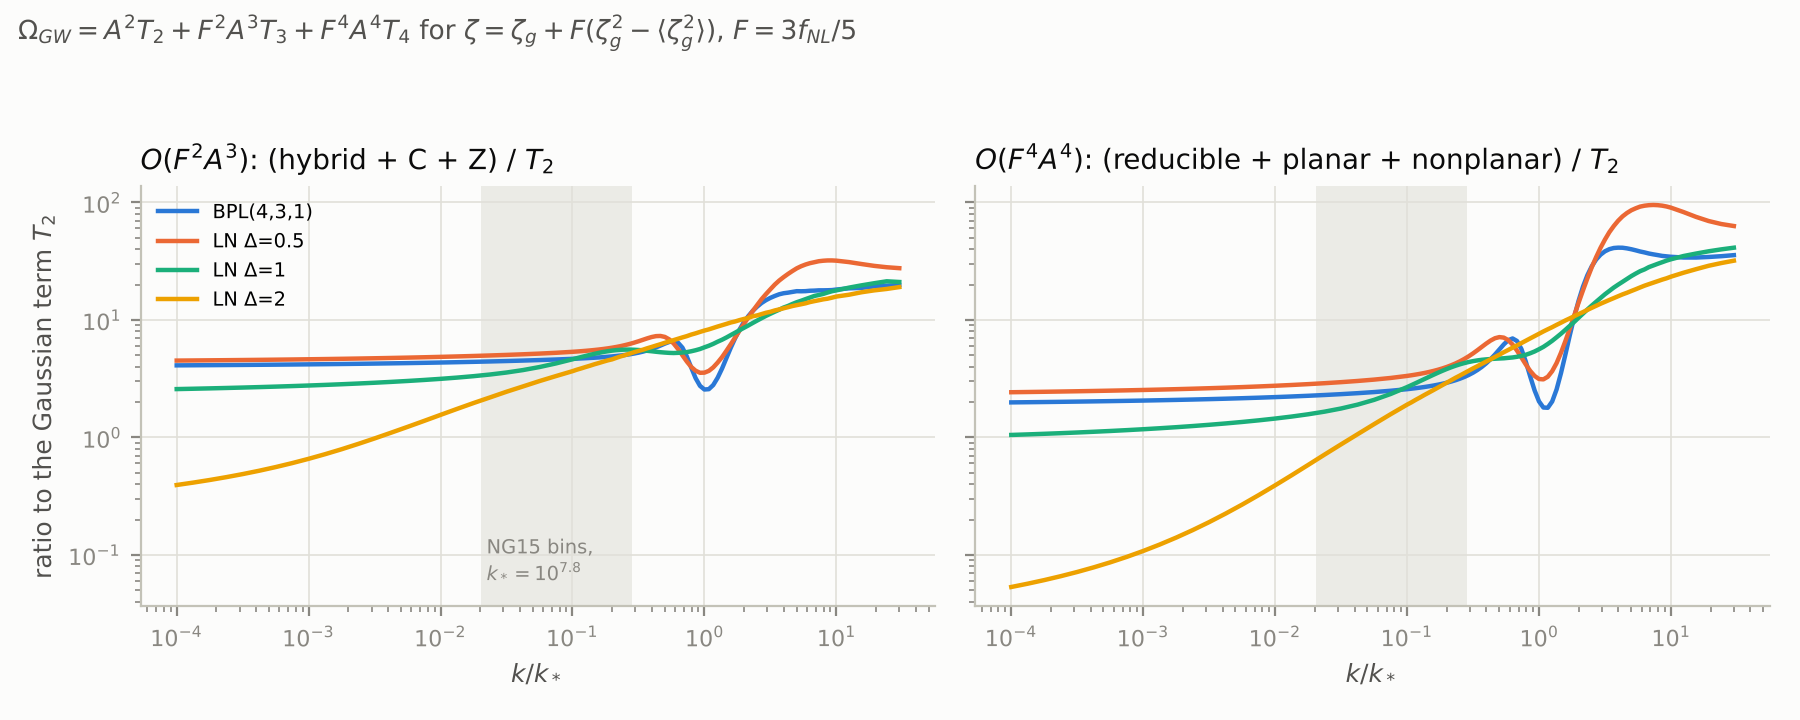
\includegraphics[width=\textwidth]{fig_sigw_ng_terms.png}
\caption{The NG corrections to the induced GW spectrum relative to the Gaussian term, per spectral
shape. Shaded: the 14 NANOGrav bins for $k_*=10^{7.8}\,{\rm Mpc}^{-1}$, near the posterior median.}
\label{fig:ngterms}
\end{figure}

\textbf{Effect on the tension.} The PBH-allowed region lies at small $A$, so the exclusion weakens
(Table~\ref{tab:ngsigw}, Fig.~\ref{fig:ngsigw}). Over the cases with $\sigma_P\le4$:
\begin{itemize}
\item $\sigma_P$ drops by 0.10--0.26 for $\fnl=\pm2$, by 0.03--0.20 for the curvaton, by
$\le0.09$ for $|\fnl|=1$, and by $\le0.03$ for $|\fnl|=0.5$ and USR $\mu_*=5/2$.
\item \textbf{The statistics shift is unchanged.} Threshold $\to$ peaks adds $+0.23$ to $+0.67$
(median $+0.39$), against $+0.24$ to $+0.68$ (median $+0.42$) with the Gaussian spectrum. None of
the 66 pairs changes by more than $\pm0.10$.
\item \textbf{The truncation matters little.} Dropping the $A^4$ terms of the quadratic template,
or adding the $F^4A^4$ terms to the others, moves $\sigma_P$ by $\le0.02$.
\end{itemize}
The GW part of the NG effect relieves the tension for either sign of $\fnl$, by at most
$0.26\sigma$. The PBH part shifts $\sigma_P$ by $-1.2$ to beyond $+2\sigma$.

\begin{table}[t]
\centering\small
\begin{tabular}{llccc}
\toprule
template & GW spectrum & BPL(4,3,1) & LN $\Delta=0.5$ & LN $\Delta=1$\\
\midrule
$\fnl=-2$ & Gaussian & 1.87\,$\to$\,2.18 & 1.88\,$\to$\,2.31 & 3.43\,$\to$\,3.84\\
 & with NG & 1.73\,$\to$\,2.05 & 1.73\,$\to$\,2.11 & 3.25\,$\to$\,3.67\\
$\fnl=-1$ & Gaussian & 1.98\,$\to$\,2.40 & 1.90\,$\to$\,2.36 & 3.05\,$\to$\,3.46\\
 & with NG & 1.94\,$\to$\,2.34 & 1.85\,$\to$\,2.30 & 2.99\,$\to$\,3.42\\
$\fnl=-0.5$ & Gaussian & 2.25\,$\to$\,2.93 & 2.22\,$\to$\,2.89 & 3.09\,$\to$\,3.51\\
 & with NG & 2.24\,$\to$\,2.91 & 2.20\,$\to$\,2.87 & 3.07\,$\to$\,3.50\\
curvaton $r_{\rm dec}=0.9$ & Gaussian & 2.01\,$\to$\,2.44 & 2.00\,$\to$\,2.43 & 3.09\,$\to$\,3.49\\
 & with NG & 1.92\,$\to$\,2.30 & 1.88\,$\to$\,2.26 & 2.95\,$\to$\,3.38\\
USR $\mu_*=5/2$ & Gaussian & 3.53\,$\to$\,$>4$ & 3.49\,$\to$\,3.91 & $>4$\\
 & with NG & 3.51\,$\to$\,4.00 & 3.47\,$\to$\,3.90 & 3.99\,$\to$\,$>4$\\
\bottomrule
\end{tabular}
\caption{$\sigma_P$ for threshold statistics $\to$ peaks of $\Cl$ with the Gaussian induced GW
spectrum (as in Table~\ref{tab:pta}) and with its primordial-NG corrections (each template with
its own posterior). $\fpbh=1$, conventions of 2306.17149. The other templates are beyond
$4\sigma$ with either spectrum.}
\label{tab:ngsigw}
\end{table}

\begin{figure}[t]
\centering
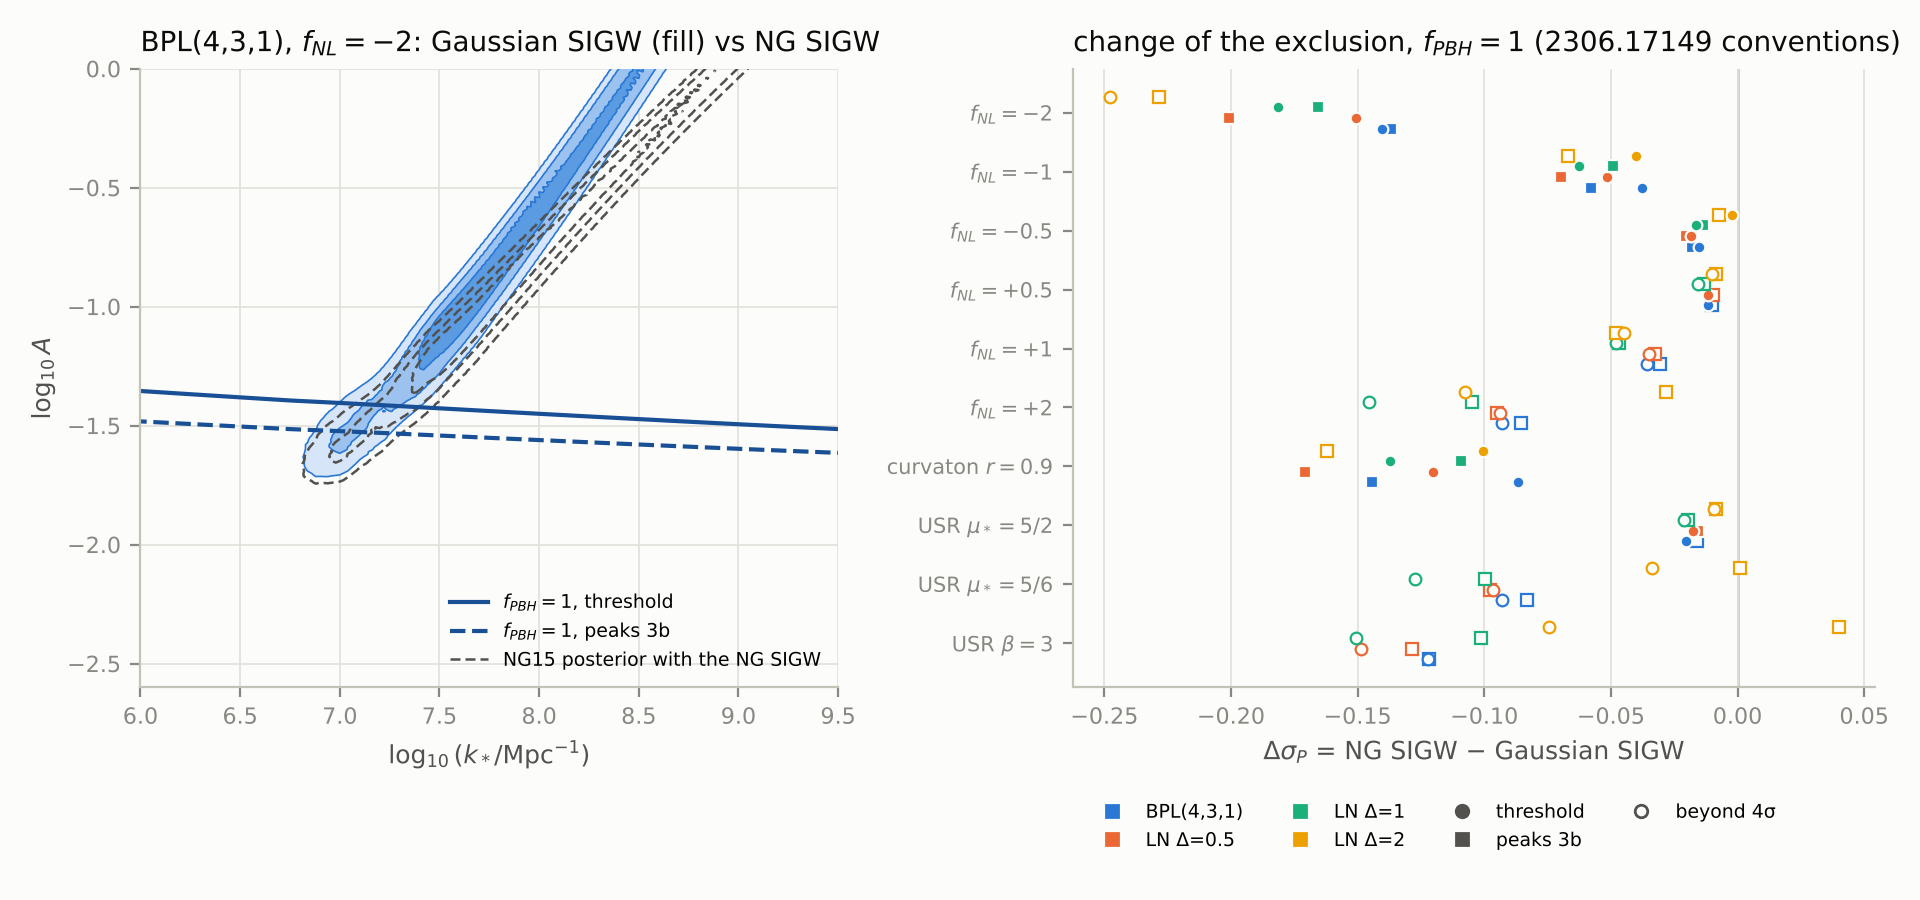
\includegraphics[width=\textwidth]{fig_phase5_ngsigw.png}
\caption{Left: the NANOGrav 15 posterior for BPL(4,3,1) with the Gaussian induced GW spectrum
(fill) and with its NG corrections for $\fnl=-2$ (dashed; 68.3/95.4/99.7\% HPD), with the $\fpbh=1$
lines. Right: the change of $\sigma_P$ from the NG corrections for every template and shape; open
symbols lie beyond $4\sigma$.}
\label{fig:ngsigw}
\end{figure}

\subsection{Robustness}

Table~\ref{tab:robust} varies one analysis choice at a time.
\begin{itemize}
\item \textbf{The statistics shift.} It survives every change: $+0.2$ to $+0.8\sigma$ across the
peak-normalisation conventions in use, and $+0.8$ to $+1.3\sigma$ with the high-peak formula.
\item \textbf{The absolute significance.} It depends mainly on the frequency range: 5, 14 or 30
bins move it by $-1.5$ to $+1\sigma$. The part of the posterior nearest the allowed region,
$k_*\simeq10^7\,{\rm Mpc}^{-1}$, places the GW peak at 10--20 nHz, and the bins above it bound it.
\item \textbf{The other conventions:}
  \begin{itemize}
  \item the transfer function in the threshold moves it by $-0.2$ to $-1.0\sigma$;
  \item the entropy-conserving $\fpbh$ normalisation by $-0.15$ to $-0.4\sigma$;
  \item $\fpbh=10^{-3}$ instead of 1 by $+0.4$ to $+0.8\sigma$.
  \end{itemize}
\item \textbf{Fixed vs marginalised shape.} Fixing the shape raises the significance relative to
marginalising over it (Gaussian BPL: $3.0$ vs $2.3\sigma_P$). The fixed BPL(4,3,1) has a steep
causality tail, which disfavours the low-$k_*$ corner closest to the allowed region.
\end{itemize}

\begin{table}[t]
\centering\small
\begin{tabular}{lcc}
\toprule
change from the reference & $\Delta\sigma_P$, threshold $\to$ peaks & max.\ change of $\sigma_P$\\
\midrule
none (14 bins, KDE blur 0.05 dex) & $+0.31$ to $+0.68$ & ---\\
prior $\log_{10}k_*\in[6,9]$, or $\log_{10}A\ge-4$ & unchanged & 0.00\\
posterior grid twice as fine & unchanged & 0.00\\
KDE blur 0, 0.03 or 0.10 dex & $+0.30$ to $+0.72$ & 0.14\\
5 frequency bins (2--10 nHz) & $+0.27$ to $+0.72$ & 1.45\\
30 frequency bins (2--59 nHz) & $+0.23$ to $+0.55$ & 1.06\\
peak volume $(2\pi)^{3/2}r^3$ & $+0.40$ to $+0.81$ & 0.14\\
Press--Schechter factor 2 & $+0.27$ to $+0.59$ & 0.09\\
\texttt{pbhstat} v0.0.6 normalisation & $+0.16$ to $+0.39$ & 0.33\\
high-peak formula \cite{Iovino24} (indicative) & $+0.82$ to $+1.29$ & 0.65\\
\bottomrule
\end{tabular}
\caption{Robustness of the PTA significances for BPL(4,3,1) and lognormals with $\Delta=0.5$ and 1,
over seven NG templates (cases with $\sigma_P\le4$). Reference prior: $\log_{10}k_*\in[5,10]$,
$\log_{10}A\in[-3,0]$.}
\label{tab:robust}
\end{table}

\section{Discussion}

\textbf{What changes.} The question we set out to answer is whether the gap between threshold
statistics and peaks theory, once local NG is included for broad spectra, changes how strongly
PBH overproduction disfavours a scalar-induced explanation of the PTA signal. It does, modestly
and uniformly.
\begin{itemize}
\item Peaks theory lowers the overproduction line by about 0.1 dex for every NG template. This
strengthens the exclusion by $\simeq0.4\sigma$, or 0.2--0.8$\sigma$ depending on the peak
normalisation.
\item The NG dependence of the gap cancels almost completely: the double ratio stays within
$\pm4\%$. NG and the choice of statistics therefore add rather than interact.
\item Negative $\fnl$ and the curvaton remain the ways to relieve the tension, but peaks theory
takes back 0.3--0.5$\sigma$ of the relief.
\item NG in the induced GWs adds power at fixed $A$. It relieves the tension by up to
$0.26\sigma$ for $|\fnl|\le2$ and does not change the gap between the statistics.
\item None of the conclusions of 2306.17149 changes qualitatively. Their footnote is correct and
now quantified.
\end{itemize}

\textbf{What dominates.} For an absolute statement about the PTA tension, the larger
uncertainties lie elsewhere. The frequency range of the fit, the treatment of the collapse
threshold and the $\fpbh$ normalisation each move the significance by about as much as the choice
of statistics, or more. All three are rarely stated. We recommend quoting them with any PBH
bound on the PTA signal, together with the peak normalisation when peaks theory is used. On the
theory side, our result says that the Gaussian-peak approximation is adequate for the PTA
question (to 0.04$\sigma$), although it miscounts peaks by up to 18\%.

\textbf{Limitations.}
\begin{itemize}
\item As in the literature we compare with, we assume spherical symmetry for the compaction of a
peak \cite{Young22}, use the mean profile (profile dispersion can matter for negative NG
\cite{Escriva26}), neglect QCD effects on the formation parameters and on the GW spectrum,
truncate the NG series of the GW spectrum at $A^3$ for the curvaton and USR maps, use
the free-spectrum refit rather than the full PTA likelihood, and ignore an astrophysical
foreground. A supermassive-black-hole-binary component would relax every tension quoted here.
\item The comparison between statistics is like-for-like, since all of these limitations affect
both statistics in the same way.
\item The absolute numbers carry the systematics of Table~\ref{tab:robust}.
\end{itemize}

\section{Conclusions}

\begin{itemize}
\item \textbf{Construction.} We have constructed peaks theory with local NG for broad spectra on
the compaction function, as the exact counterpart of threshold statistics. Maxima of the
non-Gaussian compaction are maxima of a shifted Gaussian field, corrected by a rank-one term
(eq.~\ref{eq:3b}). Monte Carlo and lattice counts confirm this.
\item \textbf{The gap.} Peaks require 18--26\% smaller amplitudes than threshold statistics. This
ratio is almost independent of NG for $|\fnl|\le2$.
\item \textbf{PTA consequence.} For NANOGrav 15 this strengthens the exclusion of a
scalar-induced explanation by 0.2--0.8$\sigma$ for every NG template. The effect is smaller than
that of NG itself for $|\fnl|\gtrsim1$ and comparable to three analysis conventions, which we
have quantified.
\item \textbf{NG in the GWs.} The primordial-NG corrections to the induced GW spectrum, all seven
terms, relieve the tension by up to $0.26\sigma$ for $|\fnl|\le2$. They leave the gap between the
statistics unchanged.
\item \textbf{Code.} \texttt{ngpbh} implements every piece and reproduces published results:
\texttt{pbhstat}, Ferrante et al., 2306.17149 and Adshead et al.
\end{itemize}

\appendix

\section{Peaks of the non-Gaussian compaction: the rank-one factor}\label{app:3b}

At a stationary point of $\Cl$, write $H_\lambda=\nabla\nabla Y_\lambda$ and $\bm g=\nabla\zr$, with
$\bm g\sim\mathcal N(0,v\mathbb I)$ independent of $H_\lambda$. The exact density is
\begin{equation}
n(c,z)=P_{\rm G}(c,z)\Big(\frac{3}{2\pi\sigma^2_{1,\lambda}}\Big)^{3/2}
\E\big[|\det(H_\lambda+\kappa\bm g\bm g^T)|\,\Theta_s\big],
\end{equation}
where $\Theta_s$ requires negative- (positive-) definiteness for $s=+1$ ($-1$). For $H\prec0$ the
matrix determinant lemma gives
$\det(-H-\kappa\bm g\bm g^T)=\det(-H)\,[1-\kappa\,\bm g^T(-H)^{-1}\bm g]$, which is linear in
$\kappa|\bm g|^2$. Averaging over the direction and length of $\bm g$ gives
$v\,\det(-H){\rm tr}(-H)^{-1}=v\,e_2(-H)$. In the BBKS shape variables
$e_2=x^2/3-(3y^2+z^2)/3$, so $f_2(x)=\E[e_2\Theta|x]$ follows from the same two-dimensional
integral as $f$; that integral reproduces BBKS's $f$ to $10^{-10}$. The interior part of the
first-order factor is then exactly $1-\tau R_2$.
\begin{itemize}
\item For $\tau>0$, maxima can only be lost, so $1-\tau R_2$ is a lower bound.
\item For $\tau<0$, configurations that become maxima add a positive $\mathcal O(\tau^2)$ term.
\end{itemize}
The Monte Carlo bounds the remainder at 0.85\% at the most extreme node tested, a shift of
0.02\% in $A_*$.

\section{The PBH abundance from entropy conservation}\label{app:fpbh}

After formation at temperature $T$, the PBH number per entropy is conserved, so
$\rho_{\rm PBH,0}=\frac34\beta\,(g_*/g_{*s})\,T\,s_0$. Here $s_0=\frac{2\pi^2}{45}g_{*s}^0T_0^3$ and
$\beta$ is the mass fraction at formation (including $\mathcal K(C-C_{\rm th})^\gamma$). With
$M_H=4\pi M_P^2/H$ and $H=\pi(g_*/90)^{1/2}T^2/M_P$ this gives
\begin{equation}
\fpbh=\frac{1}{\Omega_{\rm DM}}\int\dd\ln M_H\Big(\frac{M_H}{\Mo}\Big)^{-1/2}
\Big(\frac{g_*}{106.75}\Big)^{3/4}\Big(\frac{g_{*s}}{106.75}\Big)^{-1}\frac{\beta(M_H)}{1.0\times10^{-8}},
\end{equation}
in agreement with Carr et al.\ \cite{Carr10} to 2\%. The constant $7.9\times10^{-10}$ in eq.~(14)
of 2306.17149 makes $\fpbh$ 12.7 times larger. The form $(M_{\rm eq}/M_H)^{1/2}\beta/\Omega_{\rm DM}$
drops the factor $\Omega_m$ and the heating of the radiation by $g_{*s}$ changes after formation,
and is 3--5 times larger. Both lower the amplitude for $\fpbh=1$ by
$\ln(\text{factor})/|\ln\beta|$, i.e.\ 8--12\% at $|\ln\beta|\simeq21$.

\section{Free-spectrum density estimates}\label{app:kde}

The per-bin densities distributed with PTArcade \cite{PTArcade,Lamb} are Epanechnikov KDEs on a
grid of $10^4$ points in $\log_{10}\rho$. The kernel has compact support, so the density is
exactly zero (stored as $\ln p=-36$) outside the range of the samples. Within the sparse tails it
alternates between single-sample spikes and zero. The two most constraining bins (3.9 and
5.9 nHz) have almost no low-$\rho$ tail. Tail probabilities beyond $\sim2.5\sigma$ are therefore
lumpy and cliff-like. We replace each density by the maximum of itself and its convolution with a
0.05-dex Gaussian: the bulk is unchanged and the holes are filled. Table~\ref{tab:robust} shows
that the result changes by at most $0.14\sigma$ between no blur and 0.10 dex.

\section*{Code and data}
\texttt{ngpbh} (MIT licence) is in the accompanying repository, with:
\begin{itemize}
\item the scripts that produce every table and figure here (\texttt{README.md});
\item 91 unit tests;
\item the digitised Fig.~3 of 2306.17149 and Fig.~4 of Adshead et al.;
\item the tables of the NG terms of the induced GW spectrum per spectral shape.
\end{itemize}
The NANOGrav 15 free-spectrum densities are those of PTArcade (Zenodo record 10495907) and are
downloaded with an MD5 check.

\begin{thebibliography}{99}
\bibitem{NG15gwb} G.~Agazie {\it et al.} (NANOGrav), Astrophys.\ J.\ Lett.\ 951, L8 (2023), arXiv:2306.16213.
\bibitem{NG15np} A.~Afzal {\it et al.} (NANOGrav), Astrophys.\ J.\ Lett.\ 951, L11 (2023), arXiv:2306.16219.
\bibitem{Ananda} K.~N.~Ananda, C.~Clarkson, D.~Wands, Phys.\ Rev.\ D 75, 123518 (2007), arXiv:gr-qc/0612013.
\bibitem{Baumann} D.~Baumann, P.~J.~Steinhardt, K.~Takahashi, K.~Ichiki, Phys.\ Rev.\ D 76, 084019 (2007), arXiv:hep-th/0703290.
\bibitem{Kohri} K.~Kohri, T.~Terada, Phys.\ Rev.\ D 97, 123532 (2018), arXiv:1804.08577.
\bibitem{Espinosa} J.~R.~Espinosa, D.~Racco, A.~Riotto, JCAP 09 (2018) 012, arXiv:1804.07732.
\bibitem{Domenech} G.~Dom\`enech, Universe 7, 398 (2021), arXiv:2109.01398.
\bibitem{FIVT23} G.~Franciolini, A.~J.~Iovino, V.~Vaskonen, H.~Veerm\"ae, Phys.\ Rev.\ Lett.\ 131, 201401 (2023), arXiv:2306.17149.
\bibitem{Iovino24} A.~J.~Iovino, G.~Perna, A.~Riotto, H.~Veerm\"ae, arXiv:2406.20089.
\bibitem{IPV25} A.~J.~Iovino, G.~Perna, H.~Veerm\"ae, arXiv:2512.13648.
\bibitem{Blas26} D.~Blas, J.~W.~Foster, Y.~Gouttenoire, A.~J.~Iovino, arXiv:2602.12252.
\bibitem{Ferrante} G.~Ferrante, G.~Franciolini, A.~J.~Iovino, A.~Urbano, Phys.\ Rev.\ D 107, 043520 (2023), arXiv:2211.01728.
\bibitem{Ianniccari} A.~Ianniccari, A.~J.~Iovino, A.~Kehagias, D.~Perrone, A.~Riotto, Phys.\ Rev.\ D 109, 123549 (2024), arXiv:2402.11033.
\bibitem{BBKS} J.~M.~Bardeen, J.~R.~Bond, N.~Kaiser, A.~S.~Szalay, Astrophys.\ J.\ 304, 15 (1986).
\bibitem{Pi25} S.~Pi, M.~Sasaki, V.~Takhistov, J.~Wang, JCAP 09 (2025) 045, arXiv:2501.00295.
\bibitem{Kushwaha} A.~Kushwaha, T.~Suyama, arXiv:2603.23025.
\bibitem{ColeFumagalli} P.~S.~Cole, J.~Fumagalli, arXiv:2509.14326 (\texttt{pbhstat}).
\bibitem{Young22} S.~Young, arXiv:2201.13345.
\bibitem{Kitajima} N.~Kitajima, Y.~Tada, S.~Yokoyama, C.-M.~Yoo, arXiv:2109.00791.
\bibitem{Inui} R.~Inui {\it et al.}, arXiv:2411.07647.
\bibitem{Riccardi} F.~Riccardi, M.~Taoso, A.~Urbano, arXiv:2102.04084.
\bibitem{Escriva26} A.~Escriv\`a, arXiv:2607.08738.
\bibitem{Germani25} C.~Germani, M.~A.~Gorji, M.~Uwabo-Niibo, M.~Yamaguchi, arXiv:2503.05434.
\bibitem{Musco21} I.~Musco, V.~De Luca, G.~Franciolini, A.~Riotto, Phys.\ Rev.\ D 103, 063538 (2021), arXiv:2011.03014.
\bibitem{EGS20} A.~Escriv\`a, C.~Germani, R.~K.~Sheth, Phys.\ Rev.\ D 101, 044022 (2020), arXiv:1907.13311.
\bibitem{Saikawa} K.~Saikawa, S.~Shirai, JCAP 08 (2020) 011, arXiv:2005.03544.
\bibitem{Lamb} W.~G.~Lamb, S.~R.~Taylor, R.~van Haasteren, Phys.\ Rev.\ D 108, 103019 (2023), arXiv:2303.15442.
\bibitem{PTArcade} A.~Mitridate {\it et al.}, arXiv:2306.16377 (PTArcade).
\bibitem{ALW21} P.~Adshead, K.~D.~Lozanov, Z.~J.~Weiner, JCAP 10 (2021) 080, arXiv:2105.01659.
\bibitem{Perna24} G.~Perna, C.~Testini, A.~Ricciardone, S.~Matarrese, arXiv:2403.06962.
\bibitem{SVW06} M.~Sasaki, J.~V\"aliviita, D.~Wands, Phys.\ Rev.\ D 74, 103003 (2006), arXiv:astro-ph/0607627.
\bibitem{Carr10} B.~J.~Carr, K.~Kohri, Y.~Sendouda, J.~Yokoyama, Phys.\ Rev.\ D 81, 104019 (2010), arXiv:0912.5297.
\end{thebibliography}

\end{document}
